\chapter{Evaluation}
\label{chap:evaluation}

For demodularization to be useful, it should improve performance of modular programs.
To test whether or not this is the case, we created benchmarks to test the speed of demodularized programs versus their modular counterparts.
We also compare the results with the cross-module inliner included in Racket.
We show improvements in the size of programs through the use of a dead-code elimination algorithm.
Finally, we discuss further improvements that demodularization can enable.

\section{Racket Optimizer}

The Racket optimizer included a cross-module inliner in version 5.2. 
This inliner accomplishes many of the same improvements that the demodularizer does.
The inliner does have limitations on the size of functions that it will inline, so with large functions demodularization is still preferable.
We compare the results with the inliner turned off, with the inliner turned on, and with demodularization.
The demodularized programs are also run through the existing Racket optimizer.

\section{Testing Setup}

The tests were run on a MacBook Pro (2GHz Intel i7 processor, 8GB Memory) in OS X Yosemite, using Racket v6.2. 
Each test was run 5 times and an average of the results was taken.

\section{Micro benchmarks}

The micro benchmarks for demodularization involve a module that calls a function from another module, which calls a function from another module, and so on for the number of modules in the test. 
The function call happens in a loop to get times that are significant.
The full test generation code can be found in Appendix~\ref{chap:benchmarks}.
Figure~\ref{fig:micro-results} shows the results of running these benchmarks with different numbers of modules.
The X-axis represents the number of modules in a program.
The Y-axis represents the time in seconds it takes for the program to run, where lower times are better.
\begin{figure}
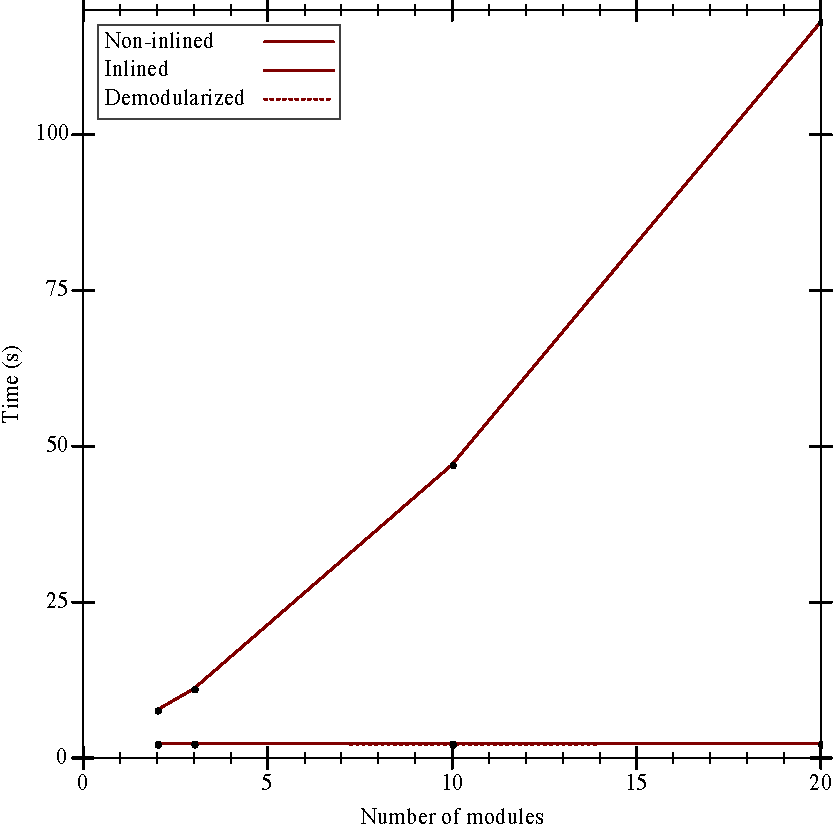
\includegraphics{figures/micro-results}
\caption{Results from micro benchmarks}
\label{fig:micro-results}
\end{figure}
Without inlining, the micro benchmarks increase in a linear fashion with an increase in the number of modules.
With inlining, the micro benchmarks stay at a constant speed.
With demodularization, the micro benchmarks also stay at a constant speed, with a slightly better speed than inlining.
Both inlining and demodularization result in similar final bytecode, where the only difference is how many times the loop is unrolled.
The cross-module inlining algorithm is more complicated than the demodularization algorithm, so there are cases where inlining would fail and demodularization would not. 
The inlining algorithm creates annotations on the bytecode of functions, which it must track and update.
If a function is too large, the algorithm will not inline it (even if it is only used once). 
Demodularization does not have these limitations because it every function in the program is available to the optimizer as if it were a local function. 
Therefore, it would be possible to create a benchmark that differentiates between cross-module inlining and demodularization by creating functions that are too large to inline, but would still be optimized in the demodularized program.

\section{Macro Benchmarks}
For macro benchmarks we selected programs that would terminate deterministically and that used multiple modules.
One of the programs we tested was a program that uses the Racket XML library to read large XML files.
The program can be found in Appendix~\ref{chap:benchmarks}.
For test data, we used astronomical data from NASA~\cite{nasa}. 
The second program we tested is a benchmark for the Redex tool.
Redex is a library that allows users to build and test semantic models.
We also tested uses of the math and plot libraries, which are written in a modular way. 
Figure~\ref{fig:macro-results} shows the results of running demodularization on larger programs.
\begin{figure}
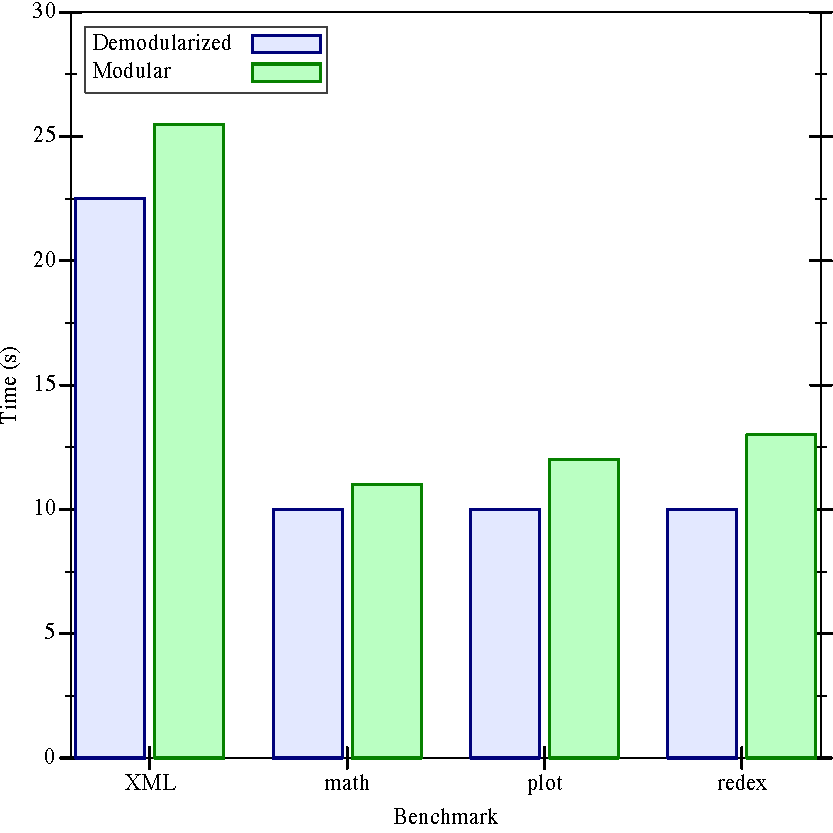
\includegraphics[width=.8\textwidth]{figures/macro-results}
\caption{Results from macro benchmarks}
\label{fig:macro-results}
\end{figure}

\section{Dead Code Elimination}
As an experiment, we implemented an unsound dead code elimination algorithm for demodularized programs.
It identifies all uses of toplevel definitions in the body of the demodularized program and eliminates all other toplevels.
The reason it is unsound is because although some toplevels may not be referenced directly in the program, they may be needed for side-effects that they have.
These side-effects may include setting up global objects or tables that will be referenced by the program, or I/O operations.
In order to make the dead code elimination algorithm sound, we would need to identify primitives that can have side-effects and include any toplevels that use those primitives.
This would be possible to do with some engineering effort, but it is beyond the scope of this work. 
The experiment gives a lower-bound on the performance of this optimization, so it is a useful result.
Figure~\ref{fig:dead-code} shows how much smaller programs become after running the dead code elimination algorithm on them.
\begin{figure}
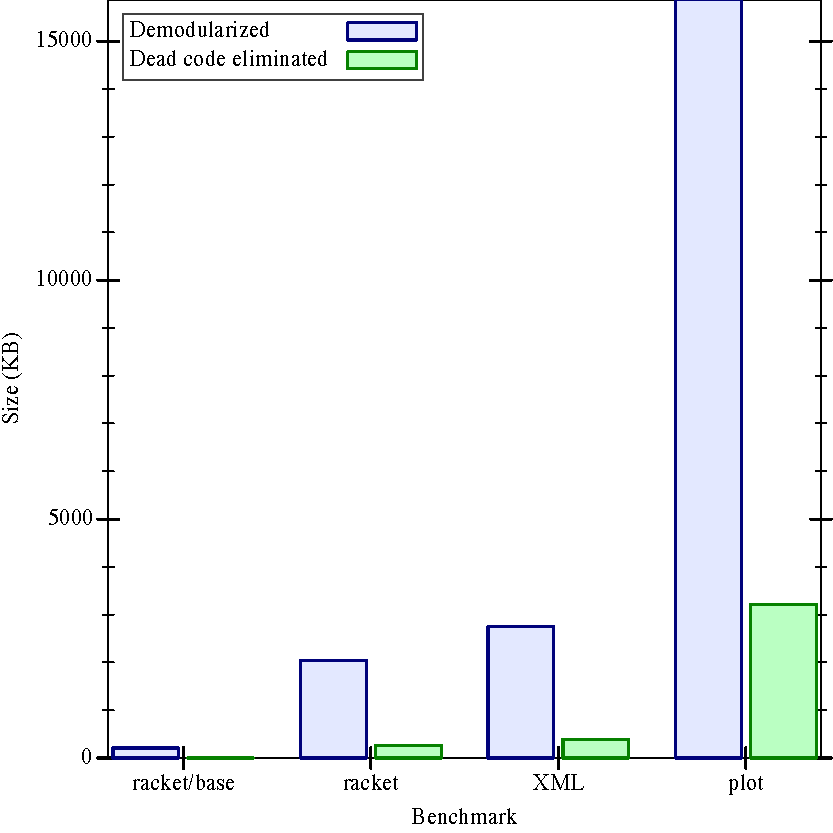
\includegraphics[width=.8\textwidth]{figures/gc-results}
\caption{Dead code elimination results}
\label{fig:dead-code}
\end{figure}
When dead code is eliminated it opens up opportunities for other optimizations because the code is smaller.
It opens up opportunities for inlining functions that are used a small number of times or determining if the values of arguments are the same.
Also, smaller code size can be a benefit by itself in space constrained or networked systems.

\section{Further Optimizations}

Having access to the whole-program at once enables optmizations that currently are not implemented by the Racket optimizer.
For example, any optimizations that rely on Control-Flow Analysis (CFA) \cite{cfa} require access to the whole program.
These include type test eliminations and inlining inside function definitions based on arguments.
Demodularization enables these sorts of optmiziations to be performed on modular programs.

Demodularization is a simple solution to the optimization problems that arise from modular programming. 
Even just using existing optimizations that were not implemented with whole programs in mind, we see some benefits in performance. 
When new optimizations are developed that take advantage of whole programs, we should see even bigger improvements in performance.
